\documentclass{beamer}

\RequirePackage{beamerthemesplit}
\RequirePackage[polish]{babel}
\RequirePackage[utf8]{inputenc}
\RequirePackage[T1]{fontenc}
\RequirePackage{times}
\RequirePackage{comment}
\RequirePackage{longtable}
\RequirePackage{url}
\RequirePackage{tabularx}
\RequirePackage{hyperref}
\RequirePackage{indentfirst}
\usepackage{listings}
\usepackage{verbatim}

\usetheme{Madrid}
\usecolortheme{seahorse}

\newtranslation[to=polish]{Section}{Część}
\newtranslation[to=polish]{Subsection}{Punkt}

\title[Zarządzanie pamięcią w Pythonie]{Zarządzanie pamięcią w Pythonie - jak działa i czy warto go dotykać?}
\subtitle{Czy w Pythonie zdarzają się wycieki pamięci? Jaki jest właściwie koszt działania garbage collectora? Kiedy mogą pojawić się problemy z pamięcią i jak możemy próbować je rozwiązać?}
% not sure if i'm allowed to put company logo on repo, so commenting it out here
%\author[Maciej Pytel]{Maciej Pytel\\ \includegraphics[height=0.2\textheight]{codi.jpg}\vspace{-4ex}}
\author[Maciej Pytel]{Maciej Pytel}
\date{02/03/2015}

\begin{document}
\selectlanguage{polish}

\begin{frame}
  \begin{titlepage}
  \end{titlepage}
\end{frame}

\begin{frame}
    \frametitle{O mnie}
    Software developer @ CodiLime. Piszę (głównie) w Pythonie. Lubię rozumieć jak rzeczy działają "w środku".
\end{frame}

\begin{frame}
    \frametitle{Disclaimer}
    \begin{block}{Który Python?}
        Ten talk jest o Pythonie 2.7.\\
        Mówiąc Python mam na myśli CPython.
    \end{block}
    \begin{block}{Przykłady}
        \url{https://github.com/MaciekPytel/python-memory-talk}
    \end{block}
\end{frame}

\section*{Plan prezentacji}
    \begin{frame}
      \tableofcontents
    \end{frame}

\setcounter{section}{0}
\section{Trochę teorii}
\frame\sectionpage
    \begin{frame}
        \frametitle{Zliczanie referencji}
        \begin{itemize}
            \item Każdy obiekt ma licznik referencji.
            \item W momencie gdy liczba referencji osiągnie 0 obiekt jest \textit{natychmiast} dealokowany.
            \item Co z cyklami referencji?
        \end{itemize}
    \end{frame}

    \begin{frame}
        \frametitle{Garbage collector}
        Zadanie: usunąć obiekty w nieosiągalnych cyklach referencji.\\
        Rozwiązanie: garbage collector.
        \begin{itemize}
            \item Uruchamiany co jakiś czas przez interpreter Pythona.
            \item Nie dealokuje obiektów, a jedynie zrywa cykle referencji.
            \item ''Zawiesza'' proces podczas zbierania śmieci.
            \item Drogi: koszt działania (co najmniej) liniowy od liczby wszystkich referencji w programie.
        \end{itemize}
    \end{frame}

    \begin{frame}
        \frametitle{Generacyjny GC}
        \begin{block}{Weak generational hypothesis}
            Większość obiektów w programie ma bardzo krótki, albo bardzo długi czas życia.
        \end{block}
        \vfill
        \begin{center}
            Czy to może nam pomóc w optymalizacji GC?
        \end{center}
    \end{frame}

    \begin{frame}
        \frametitle{Generacyjny GC}
        \begin{itemize}
            \item Dzielimy obiekty na 3 generacje (0, 1, 2).
            \item Każdy nowo alokowany obiekt trafia do generacji 0.
            \item Dłużej istniejące obiekty znajdują się w wyższych generacjach.
            \item Na generację 0 składa się niedużo obiektów, które z dużym prawdopodobieństwem można zwolnić (zgodnie z hipotezą powyżej).
        \end{itemize}
    \end{frame}

    \begin{frame}
        \frametitle{Generacyjny GC}
        \begin{itemize}
            \item Garbage collection n-tej generacji to taki, w którym GC przeanalizował obiekty generacji 0..n.
            \item Obiekt, który przeżył GC n-tej generacji jest promowany do generacji n + 1 (technicznie min(2, n + 1)).
            \item GC generacji 0 jest tanie - przeprowadzamy je często.
            \item GC wyższych generacji są droższe - przeprowadzamy je znacznie rzadziej.
        \end{itemize}
    \end{frame}

    \begin{frame}
        \frametitle{Słabe referencje}
        \begin{itemize}
            \item Referencje nie zwiększające licznika referencji wskazywanego przez siebie obiektu.
            \item Istnienie słabej referencji nie zapobiega dealokacji obiektu.
            \item W Pythonie dostarczane przez moduł \textit{weakref}.
            \item Dereferencja słabej referencji do zwolnionego obiektu zwraca None.
        \end{itemize}
    \end{frame}


\section{Czemu warto o tym wszystkim wiedzieć? Co i jak możemy zrobić?}
\frame\sectionpage
\subsection{Przykład: RESTful server}
\frame\subsectionpage
    \begin{frame}
        \frametitle{Opis eksperymentu}
        \begin{itemize}
            \item Serwer:
            \begin{itemize}
                \item Flask-RESTful + gunicorn.
                \item Dwie klasy: Task i Subtask.
                \item Relacja jeden-do-wielu (każdemu Taskowi odpowiada wiele Subtasków).
                \item API pozwala dodawać, odczytywać i usuwać Taski i Subtaski.
            \end{itemize}
            \item Test: uruchomić kilku klientów wysyłających w pętli żądania i mierzyć wydajność.
        \end{itemize}
    \end{frame}

    \begin{frame}[fragile]
        \frametitle{Task}
        \begin{semiverbatim}
class Task(object):
    def __init__(self, name):
        self.name = name
        self._subtasks = \{\}

    def add_subtask(self, name):
        self._subtasks[name] = Subtask(name, self)

    def get_subtask(self, name):
        return self._subtasks.get(name, None)
        \end{semiverbatim}
\end{frame}
% the above can't be intended or it won't compile, wtf :s

    \begin{frame}[fragile]
        \frametitle{Subtask wersja 1}
        \begin{semiverbatim}
class Subtask(object):
    def __init__(self, name, task):
        self.name = name
        self._task = task

    def get_task(self):
        return self._task
        \end{semiverbatim}
\end{frame}
% the above can't be intended or it won't compile, wtf :s

    \begin{frame}
        \frametitle{REST API}
        \begin{itemize}
            \item \textbf{GET /tasks/\{task\_id\}/} - zwróć listę Subtasków powiązanych z Taskiem o danym id (JSON)
            \item \textbf{PUT /tasks/\{task\_id\}/} - stwórz Task o zadanym id
            \item \textbf{DELETE /tasks/\{task\_id\}/} - usuń Task i wszystkie jego Subtaski
            \item \textbf{GET /subtasks/\{subtask\_id\}/} - zwróć Task, do którego przypisany jest dany Subtask
            \item \textbf{PUT /subtasks/\{task\_id\}/\{subtask\_id\}} - stwórz Subtask o danym id i przypisz do Taska o danym id
        \end{itemize}
    \end{frame}

    \begin{frame}
        \frametitle{Wyniki}
        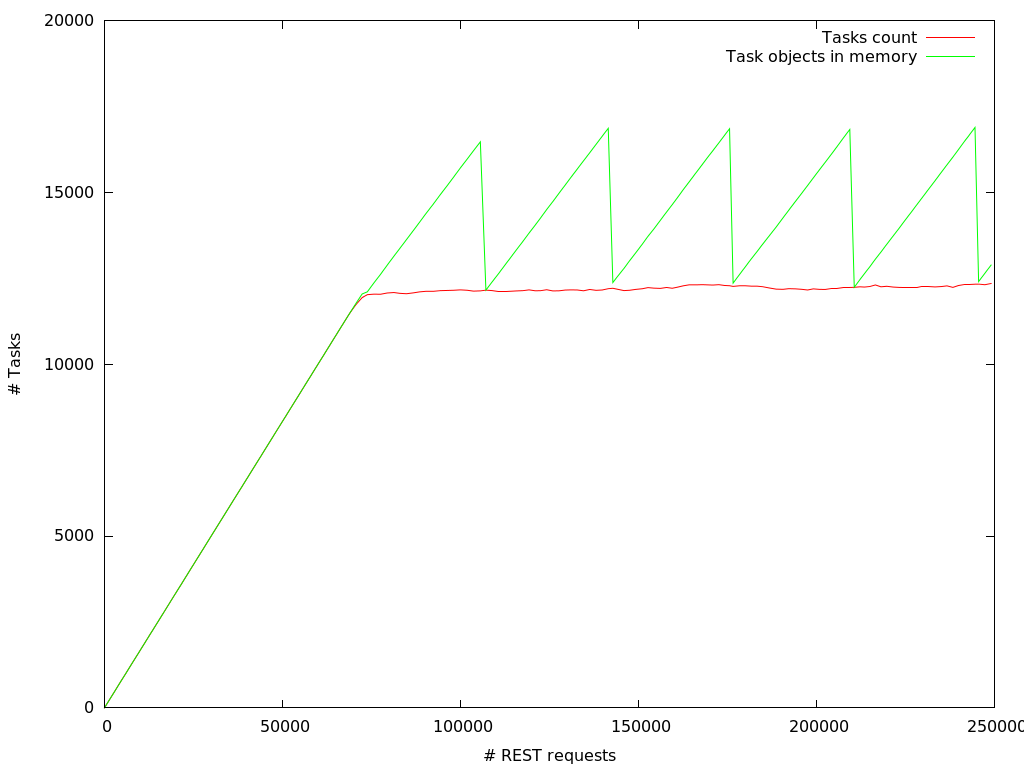
\includegraphics[height=0.8\textheight]{gc_tasks.png}
    \end{frame}

    \begin{frame}[fragile]
        \frametitle{Subtask wersja 2}
        \begin{semiverbatim}
import weakref

class Subtask(object):
    def __init__(self, name, task):
        self.name = name
        \alert{self._task = weakref.ref(task)}

    def get_task(self):
        return self._task()

        \end{semiverbatim}
\end{frame}
% the above can't be intended or it won't compile, wtf :s

    \begin{frame}
        \frametitle{Efekty?}
        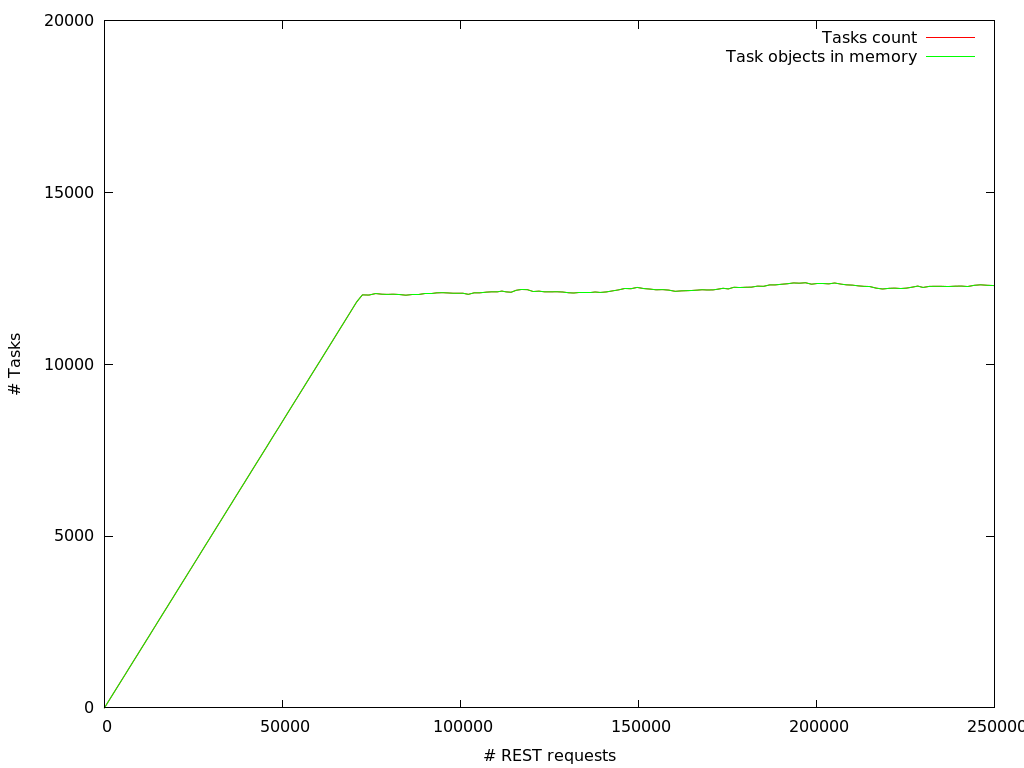
\includegraphics[height=0.8\textheight]{wr_tasks.png}
    \end{frame}

    \begin{frame}
        \frametitle{Efekty cd.}
        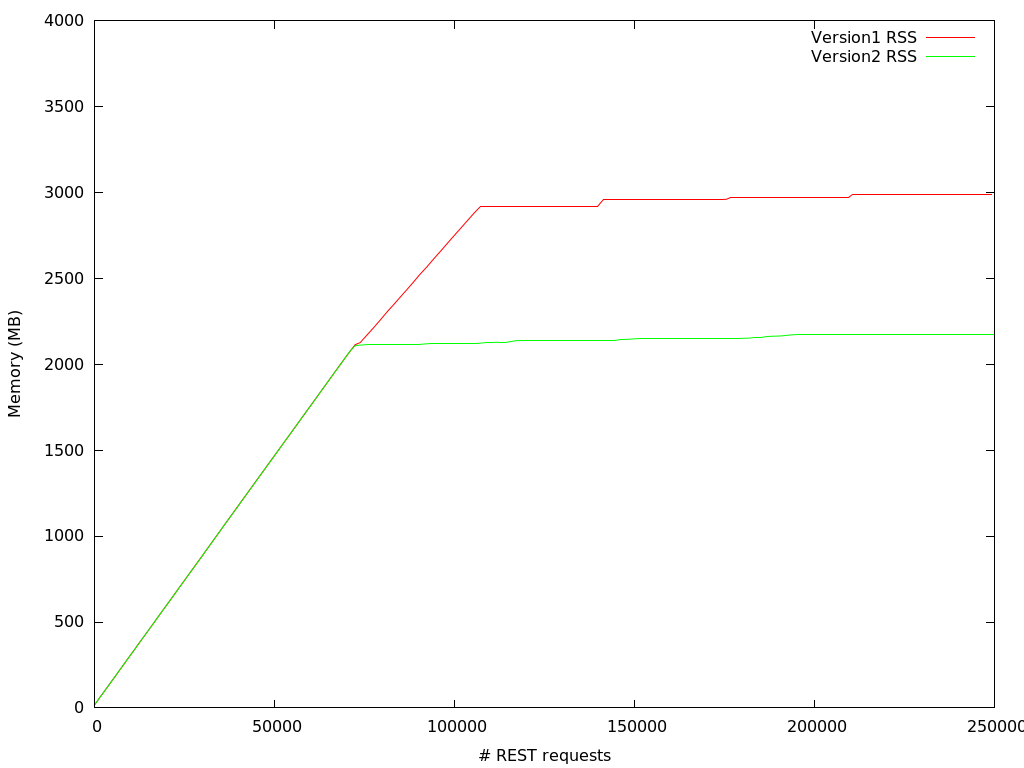
\includegraphics[height=0.8\textheight]{mem_usage.png}
    \end{frame}

    \begin{frame}
        \frametitle{Efekty cd.}
        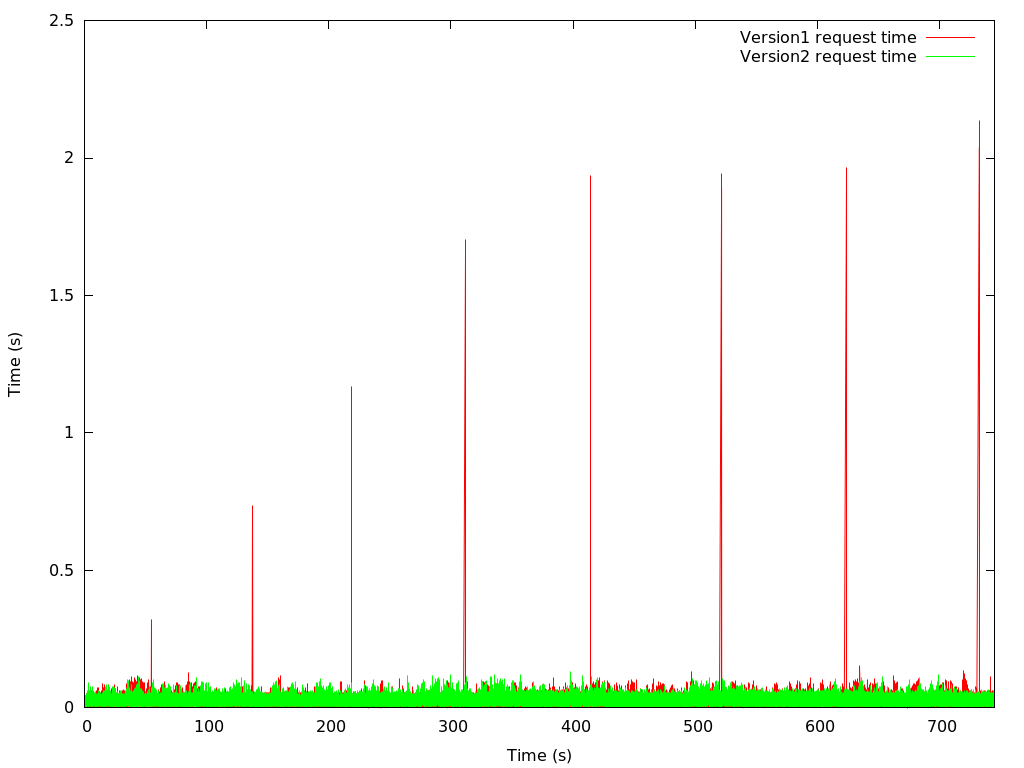
\includegraphics[height=0.8\textheight]{request_time.png}
    \end{frame}

    \begin{frame}
        \frametitle{Wnioski}
        \begin{itemize}
            \item Poleganie na GC jest kosztowne.
            \item W szczególności GC drugiej generacji trwa naprawdę długo (2-2.5s dla serwera z przykładu).
            \item Koszt wywołań GC niższych generacji jest wyraźnie niższy (nie widać wyraźnego wpływu na czas odpowiedzi serwera).
            \item GC drugiej jest uruchamiany bardzo rzadko.
            \item Python potrafi ponownie używać zwolnioną pamięć, ale nie wydaje się jej zwracać do systemu operacyjnego.
        \end{itemize}
    \end{frame}

    \begin{frame}
        \frametitle{Zwalnianie pamięci}
        \begin{itemize}
            \item Python ma własny alokator pamięci (szczegóły wychodzą poza zakres tego talka).
            \item Alokator potrafi zwracać pamięć do kernela\textsuperscript{*}, ale:
            \begin{itemize}
                \item Pamięć jest alokowana w blokach i będzie zwrócona tylko gdy cały blok jest wolny (fragmentacja!).
                \item Dla wielu obiektów (np. tuple) zwalniane obiekty trafiają do puli, do ponownego użycia.
                \item Pamięć raz zarezerwowana na inty nigdy nie będzie użyta na nic innego.
                \item To samo dla floatów.
                \item ...
            \end{itemize}
        \end{itemize}
    \end{frame}

    \begin{frame}
        \frametitle{Ogólne wnioski}
        Jeśli mamy problemy ze zużyciem pamięci przez nasz program:
        \begin{itemize}
            \item Warto usuwać referencje do obiektów natychmiast, gdy przestaną być potrzebne.
            \item Warto unikać \textit{zbędnych} cykli referencji przy pisaniu aplikacji.
            \item W większości pozostałych przypadków da się użyć słabych referencji.
            \item Albo explicite zrywać cykle referencji gdy obiekty przestaną być potrzebne (np. definiując i wołając metodę \textit{delete}).
            \item \textit{xrange} zamiast \textit{range} w długich pętlach robi różnicę. Serio.
        \end{itemize}
    \end{frame}

\subsection{Wycieki pamięci}
\frame\subsectionpage

    \begin{frame}
        \frametitle{Wycieki pamięci}
        Jest kilka możliwych przyczyn wycieku pamięci:
        \begin{enumerate}
            \item Wyciek pamięci w module napisanym w c/c++.
            \item Pamięć przeznaczona na inty, lub floaty nigdy nie będzie zwolniona, lub przeznaczona na cokolwiek innego.
            \item Trzymanie ''zapomnianych'' referencji do struktur danych.
            \item Garbage collector nie zwolni \textit{żadnego} obiektu będącego częścią cyklu, w którym choć jeden obiekt definiuje finalizer (\textit{\_\_del\_\_}).
        \end{enumerate}
    \end{frame}

    \begin{frame}
        \frametitle{''Zapomniane'' referencje}
        Warto pamiętać o kilku nieoczywistych miejscach w których mogą pozostać referencje do naszych obiektów:
        \begin{enumerate}
            \item sys.exc\_info() zwraca informacje o ostatnim wyjątku obsłużonym w obecnej ramce (frame) stosu. Jedną z informacji jest obiekt traceback zawierający cały stan stosu w momencie rzucenia wyjątku. Ups.
            \item Domknięcia, functools.partial, itp.
        \end{enumerate}
    \end{frame}

    \begin{frame}
        \frametitle{Finalizer (\_\_del\_\_)}
        \begin{itemize}
            \item Jeśli obiekt definiuje metodę \_\_del\_\_ zostanie ona wywołana tuż przed dealokacją obiektu.
            \item W \_\_del\_\_ obiekt może stworzyć referencję do siebie - zapobiegnie to jego usunięciu.
            \item \textbf{GC nigdy nie zdealokuje obiektu, który ma zdefiniowane \_\_del\_\_!}
            \item Innymi słowy cykl referencji w którym występuje obiekt ze zdefiniowanym \_\_del\_\_ nie zostanie nigdy zerwany.
            \item \textbf{Uwaga:} \_\_del\_\_ jest używany w wielu bibliotekach (a nawet w standardowej bibliotece Pythona!).
        \end{itemize}
    \end{frame}

    \begin{frame}
        \frametitle{Finalizer c.d.}
        Jak widać finalizer tworzy problemy? Jak je rozwiązać?
        \begin{itemize}
            \item Nie używać. Context manager ("with") jest prawie zawsze lepszym rozwiązaniem.
            \item Jeśli potrzebujemy finalizera - upewnić się że obiekt, który definiuje finalizer nie jest w cyklu referencji (dekompozycja).
            \item W ostateczności: weakref.ref przyjmuje jako opcjonalny parametr callback, który zostanie wywołany po usunięciu obiektu. Problem: obiekt jest już usunięty w momencie wywołania callbacku, więc musimy gdzieś przechować stan potrzebny tej funkcji.
        \end{itemize}
    \end{frame}

    \begin{frame}[fragile]
        \frametitle{Finalizer przy użyciu weakref}
        \begin{semiverbatim}
class FileWrapper(object):
    _weakrefs = set()

    @classmethod
    def _delegated_close(cls, file_object, w):
        file_object.close()
        cls._weakrefs.remove(w)

    def __init__(self, name, mode):
        self._f = open(name, mode)
        self._weakrefs.add(weakref.ref(
            self,
            functools.partial(self._delegated_close,
                self._f)))
        \end{semiverbatim}
\end{frame}

\section{Kilka przydatnych narzędzi}
\frame\sectionpage

    \begin{frame}
        \frametitle{pdb}
        \begin{center}
            Debugger, część standardowej biblioteki Pythona. Pozwala poruszać się po stosie, wykonywać kod i ewaluować wyrażenia w kontekście dowolnej ramki, analizować wyjątki, ...
        \end{center}
    \end{frame}

    \begin{frame}
        \frametitle{gc}
        Moduł ze standardowej biblioteki Pythona.
        \begin{itemize}
            \item \textbf{gc.collect(generation=2)} - ręczne wywołanie GC.
            \item \textbf{gc.enable() / gc.disable()} - włącz/wyłącz automatyczne GC.
            \item \textbf{gc.garbage} - lista wszystkich obiektów, które powinny zostać zwolnione, ale mają zdefiniowane \_\_del\_\_.
            \item Pozwala ustawić flagi dla garbage collectora, powodujące np. wypisanie statystyk po zakończeniu GC.
            \item Potrafi podać listę wszystkich obiektów trzymających referencję do naszego obiektu.
        \end{itemize}
    \end{frame}

    \begin{frame}
        \frametitle{objgraph}
        Biblioteka do analizy obiektów w pamięci i szukania wycieków pamięci.
        \begin{itemize}
            \item Dostępna przez pip.
            \item Wizualizacja grafów referencji pomiędzy obiektami.
            \item Informacja o liczbie obiektów poszczególnych typów w pamięci.
            \item Zmiana ilości obiektów danego typu w czasie.
            \item Wystarcza do zdiagnozowania 99\% problemów.
        \end{itemize}
    \end{frame}

    \begin{frame}
        \frametitle{objgraph}
        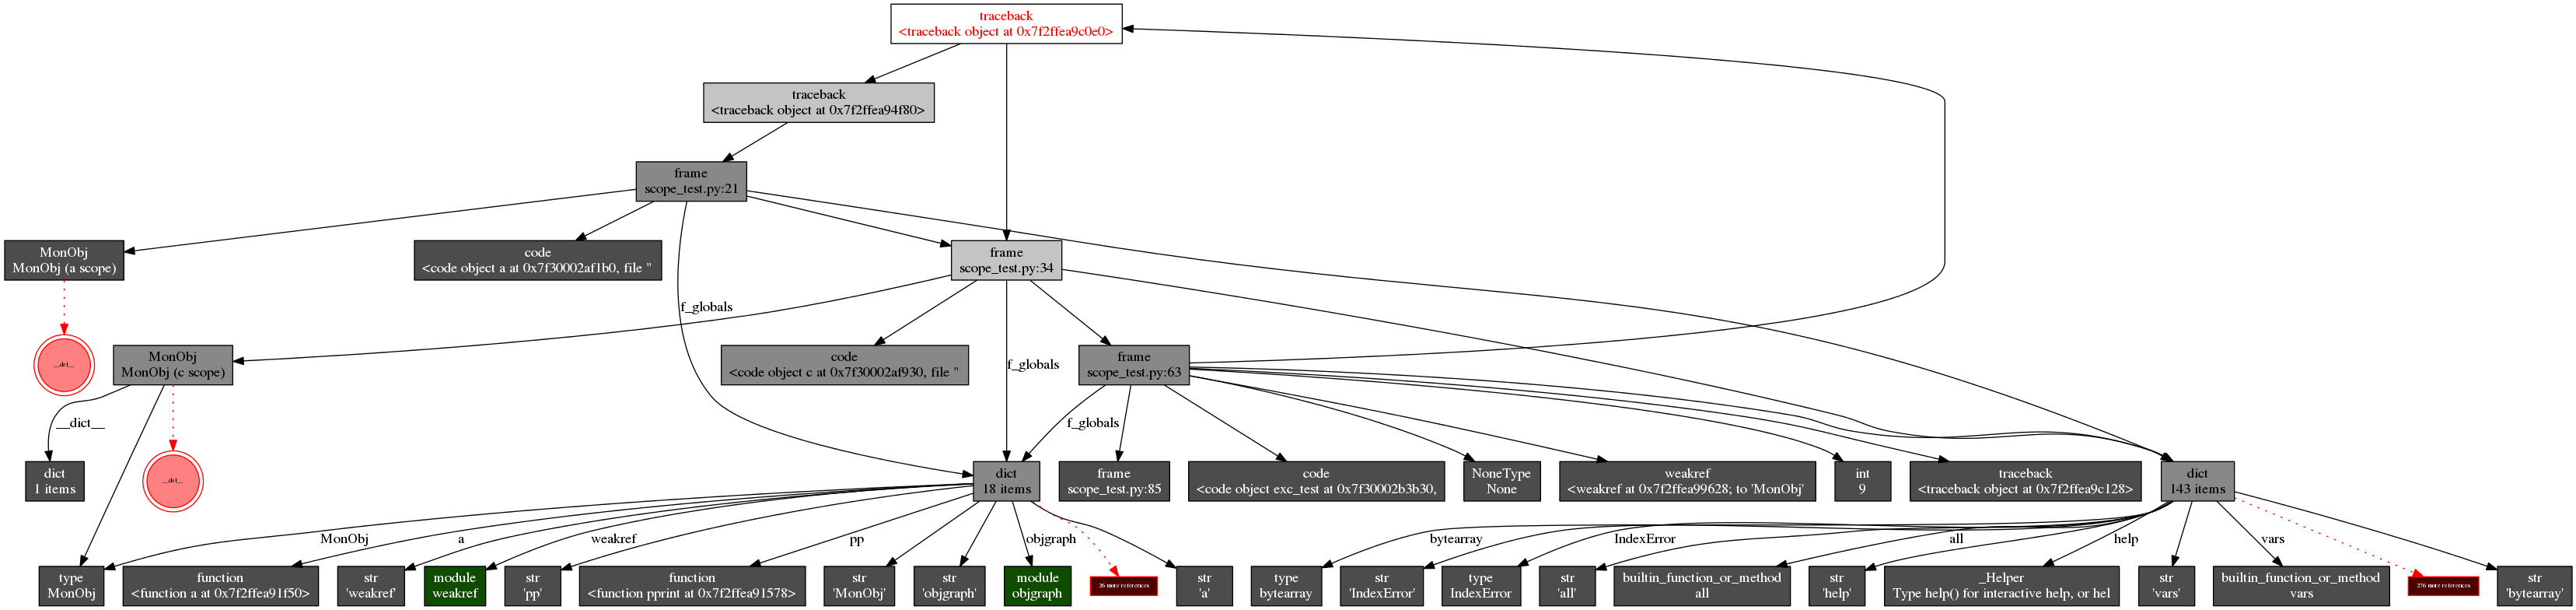
\includegraphics[height=0.3\textheight]{objgraph_example.png}
    \end{frame}

    \begin{frame}
        \frametitle{guppy/heapy}
        \begin{itemize}
            \item Narzędzie do profilowania i analizy problemów z pamięcią.
            \item Mnóstwo funkcji: analiza ścieżek w grafie zależności, drzewa rozpinające grafu referencji (!), grupowanie obiektów według różnych relacji równoważności (np. klasa, moduł z którego pochodzą), ...
            \item Da się dodać śledzenie własnych obiektów z modułu napisanego w C.
            \item Nienajlepsza dokumentacja i brak dobrych tutoriali w sieci.
            \item Na ten 1\% sytuacji, gdy objgraph nie wystarczy :)
        \end{itemize}
    \end{frame}

\section{Trochę więcej teorii, czyli jak to właściwie działa}
\frame\sectionpage

    \begin{frame}
        \frametitle{Generacje}
        \begin{itemize}
            \item Każda generacja jest listą dwukierunkową.
            \item Nowo alokowany obiekt jest dodawany do generacji 0.
            \item Przed GC n-tej generacji listy obiektów niższych generacji są doklejane do listy obiektów n-tej generacji.
            \item Po GC n-tej generacji lista żywych obiektów jest doklejana do listy obiektów generacji n + 1.
        \end{itemize}
    \end{frame}

    \begin{frame}
        \frametitle{Algorytm GC}
        \begin{enumerate}
            \item (Dla generacji 1 i 2) Dołącz obiekty niższych generacji (scalanie list dwukierunkowych).
            \item Przeiteruj po obiektach na liście. Sprawdź wychodzące z nich referencje i jeśli prowadzą do innych obiektów na liście zmniejsz licznik referencji tych obiektów.
            \item Przeiteruj po obiektach na liście. Jeśli ich licznik referencji wynosi 0 przenieś je na listę \textit{unreacheable}.
            \item Przeiteruj po obiektach pozostałych na liście. Sprawdź wychodzące z nich referencje i przenieś z powrotem każdy bezpośrednio osiągalny obiekt na liście \textit{unreacheable}.
            \item Przywróć oryginalne wartości liczników referencji.
            \item Dołącz listę osiągalnych obiektów do listy obiektów generacji n + 1.
            \item Usuń wszystkie referencje wychodzące z obiektów na liście \textit{unreacheable}.
        \end{enumerate}
    \end{frame}

    \begin{frame}
        \frametitle{Przykład}
        \begin{center}
            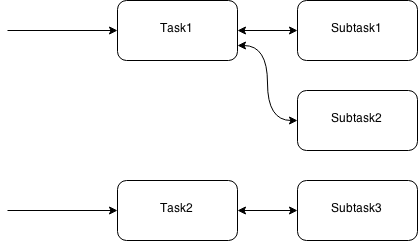
\includegraphics[height=0.5\textheight]{graph_initial.png}
        \end{center}
    \end{frame}

    \begin{frame}
        \frametitle{Przykład}
        \begin{center}
            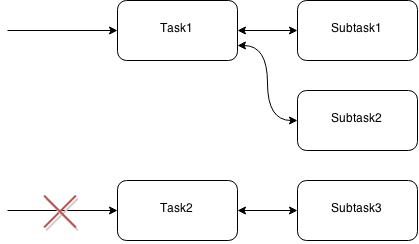
\includegraphics[height=0.5\textheight]{graph_remove.png}
        \end{center}
    \end{frame}

    \begin{frame}
        \frametitle{GC - wizualizacja}
        \begin{center}
            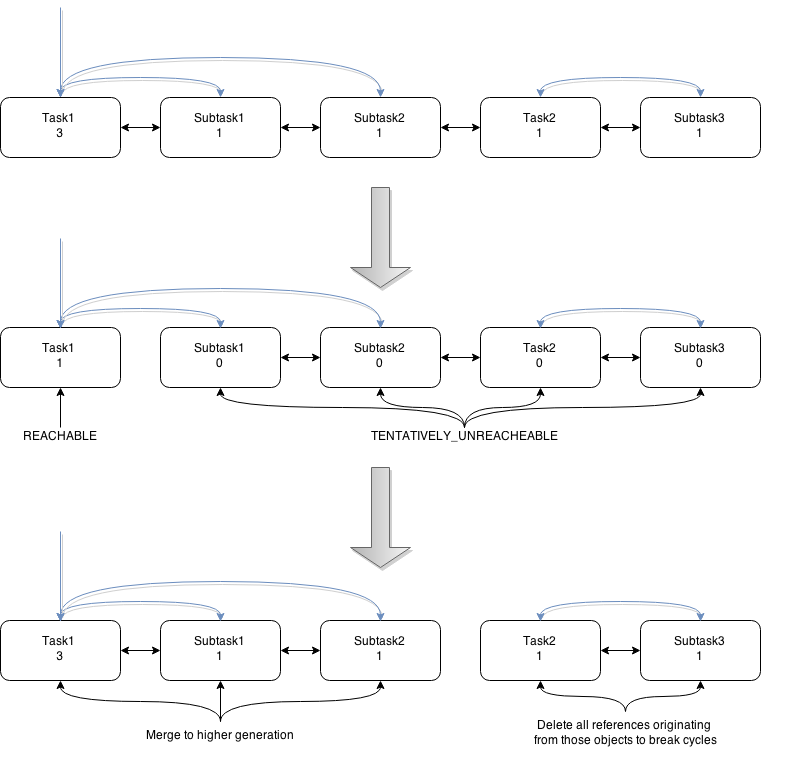
\includegraphics[height=0.8\textheight]{full_gc_drawing.png}
        \end{center}
    \end{frame}

    \begin{frame}
        \frametitle{Uwagi}
        \begin{itemize}
            \item Przedstawiany algorytm oddaję ogólną ideę działania GC w Pythonie. Rzeczywista implementacja jest trochę bardziej skomplikowana.
            \item Szczegóły w kodzie źródłowym Pythona, plik /Modules/gcmodule.c - bardzo dużo komentarzy.
        \end{itemize}
    \end{frame}

    \begin{frame}
        \frametitle{Cytat na koniec}
        \begin{quote}
            Programmers waste enormous amounts of time thinking
            about the speed of noncritical parts of their programs (...). We
            should forget about small efficiencies, say about 97\% of the
            time: premature optimization is the root of all evil. Yet we
            should not pass up our opportunities in that critical 3\%.
        \end{quote}
        \hspace*\fill{- Donald Knuth}
    \end{frame}

\end{document}
